\documentclass[12pt]{article}

% ---- Fonts ----
\usepackage{mathptmx}   % Times New Roman for text and math
\usepackage[T1]{fontenc}
\usepackage[utf8]{inputenc}

% ---- Layout ----
\usepackage[a4paper,margin=1in]{geometry}
\usepackage{setspace}
\onehalfspacing

% ---- Graphics and captions ----
\usepackage{graphicx}
\usepackage{float}
\usepackage{caption}
\captionsetup{font=small,labelfont=bf,justification=centering}
\graphicspath{{images/}}

% ---- Links and references ----
\usepackage[hidelinks]{hyperref}

% ---- Headings ----
\usepackage{titlesec}
\titleformat{\section}{\normalfont\Large\bfseries}{\thesection.}{0.6em}{}
\titleformat{\subsection}{\normalfont\large\bfseries}{\thesubsection}{0.6em}{}

% ---- Colors (for the cover only) ----
\usepackage{xcolor}

\begin{document}

% =====================================================
% COVER PAGE
% =====================================================
\begin{titlepage}
    \centering
    \vspace*{1cm}

    
\includegraphics[width=0.45\textwidth]{diyar-logo.jpg}

    \vspace{2.5cm}

    {\Huge\bfseries HR Automation Project\par}
    \vspace{0.5cm}
    {\Large Progress Report and Path to Finalization\par}

    \vspace{2.5cm}

    \begin{tabular}{rl}
        \textbf{Prepared for:} & Diyar Management \\[0.3em]
        \textbf{Prepared by:}  & Jassem El Danaf \\[0.3em]
        \textbf{Date:}         & April 2026 \\[0.3em]
        \textbf{Status:}       & Proof of concept, work in progress \\
    \end{tabular}

    \vfill

    {\small An end-to-end internal HR pipeline covering job openings, AI-assisted CV evaluation, shortlisting, and candidate communication. Runs entirely on a local machine with no cloud dependencies.}

    \vspace{1cm}
\end{titlepage}

% =====================================================
% TABLE OF CONTENTS
% =====================================================
\tableofcontents
\newpage

% =====================================================
% EXECUTIVE SUMMARY
% =====================================================
\section{Executive Summary}

The Diyar HR Automation project is at a proof-of-concept stage. It is not a finished product yet, but it is a working prototype that an HR user can open in a browser and drive from end to end, covering five connected stages: dashboard, job openings, AI-assisted CV evaluation, shortlisting, and candidate emails. Everything runs locally on one machine, so there are no hosting costs and no candidate data leaves the company. This report summarizes what has been built, how the pieces fit together, and the work still ahead before the project can be considered complete.

% =====================================================
% ARCHITECTURE
% =====================================================
\section{System Architecture}

The solution is built from four cooperating pieces, each with a narrow responsibility. The browser talks only to n8n; n8n talks to the database, the AI model, and a small Python helper that sends emails. This keeps each layer simple and replaceable.

\begin{table}[H]
    \centering
    \begin{tabular}{|p{4.2cm}|p{10cm}|}
        \hline
        \textbf{Component} & \textbf{Role} \\
        \hline
        Frontend (web UI) & Single HTML file with all pages, wizards, and tables. The HR user opens it in a browser with nothing to install. \\
        \hline
        n8n workflows & Visual automation engine that exposes webhooks to the browser, queries the database, and calls the AI model. Plays the role of a backend without needing one written from scratch. \\
        \hline
        PostgreSQL (Docker) & Stores every job opening, candidate, evaluation, shortlist entry, and email record. \\
        \hline
        Local AI model (Ollama, qwen3:4b) & Generates job descriptions, drafts evaluation criteria, and scores CVs. All inference runs on the laptop. \\
        \hline
        SMTP helper (Python) & Small local service that sends outbound email and reports delivery status back to n8n. \\
        \hline
    \end{tabular}
    \caption{The five components of the HR Automation system and what each one is responsible for.}
\end{table}

% =====================================================
% INFRASTRUCTURE LAYER
% =====================================================
\section{Infrastructure Layer}

\subsection{Docker and PostgreSQL}

PostgreSQL runs inside a Docker container named \texttt{hr-postgres}. Docker keeps the database isolated from the host machine and makes setup a single command. Anyone who needs to reproduce the environment on a new laptop can do so in minutes.

\begin{figure}[H]
    \centering
    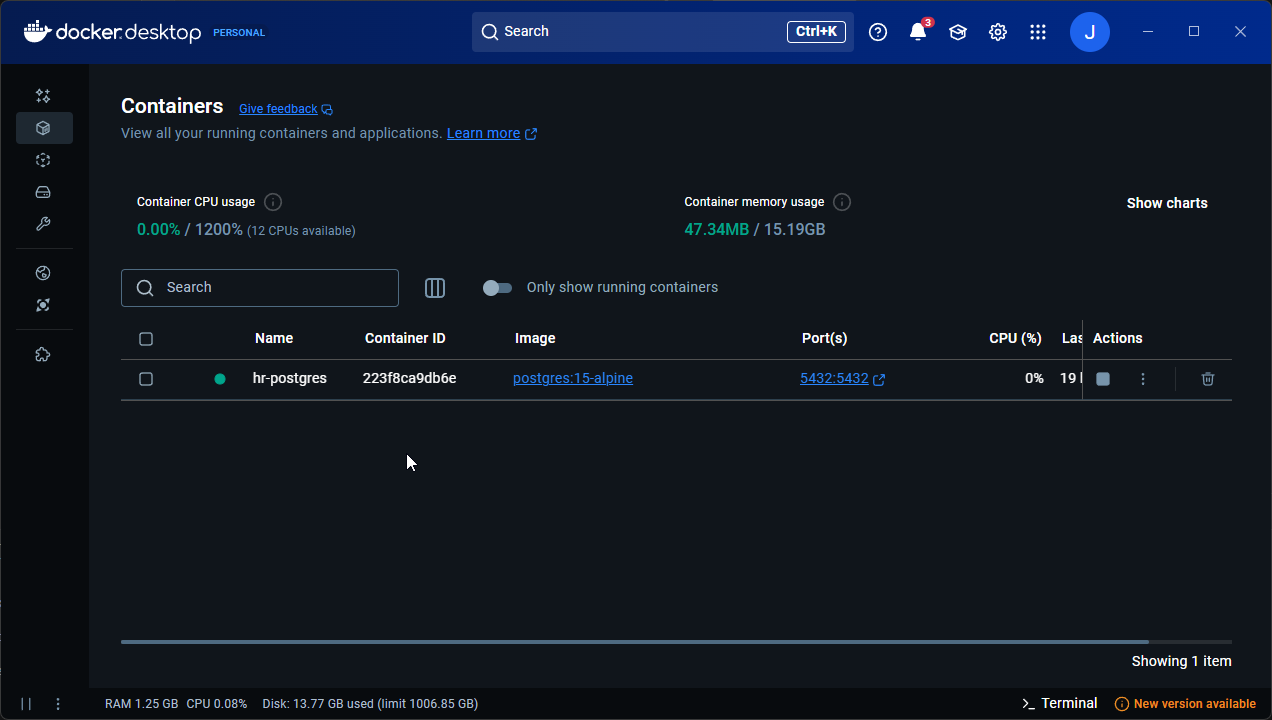
\includegraphics[width=0.9\textwidth]{docker.png}
    \caption{Docker Desktop showing the \texttt{hr-postgres} container running on port 5432. This is the only container the project uses, which keeps operations straightforward.}
\end{figure}

\subsection{n8n as the Orchestration Layer}

Instead of writing a custom backend from scratch, the project uses n8n. Every browser request hits an n8n webhook, which then runs a small pipeline of steps such as validating input, reading or writing the database, calling the AI model, or sending an email.

\begin{figure}[H]
    \centering
    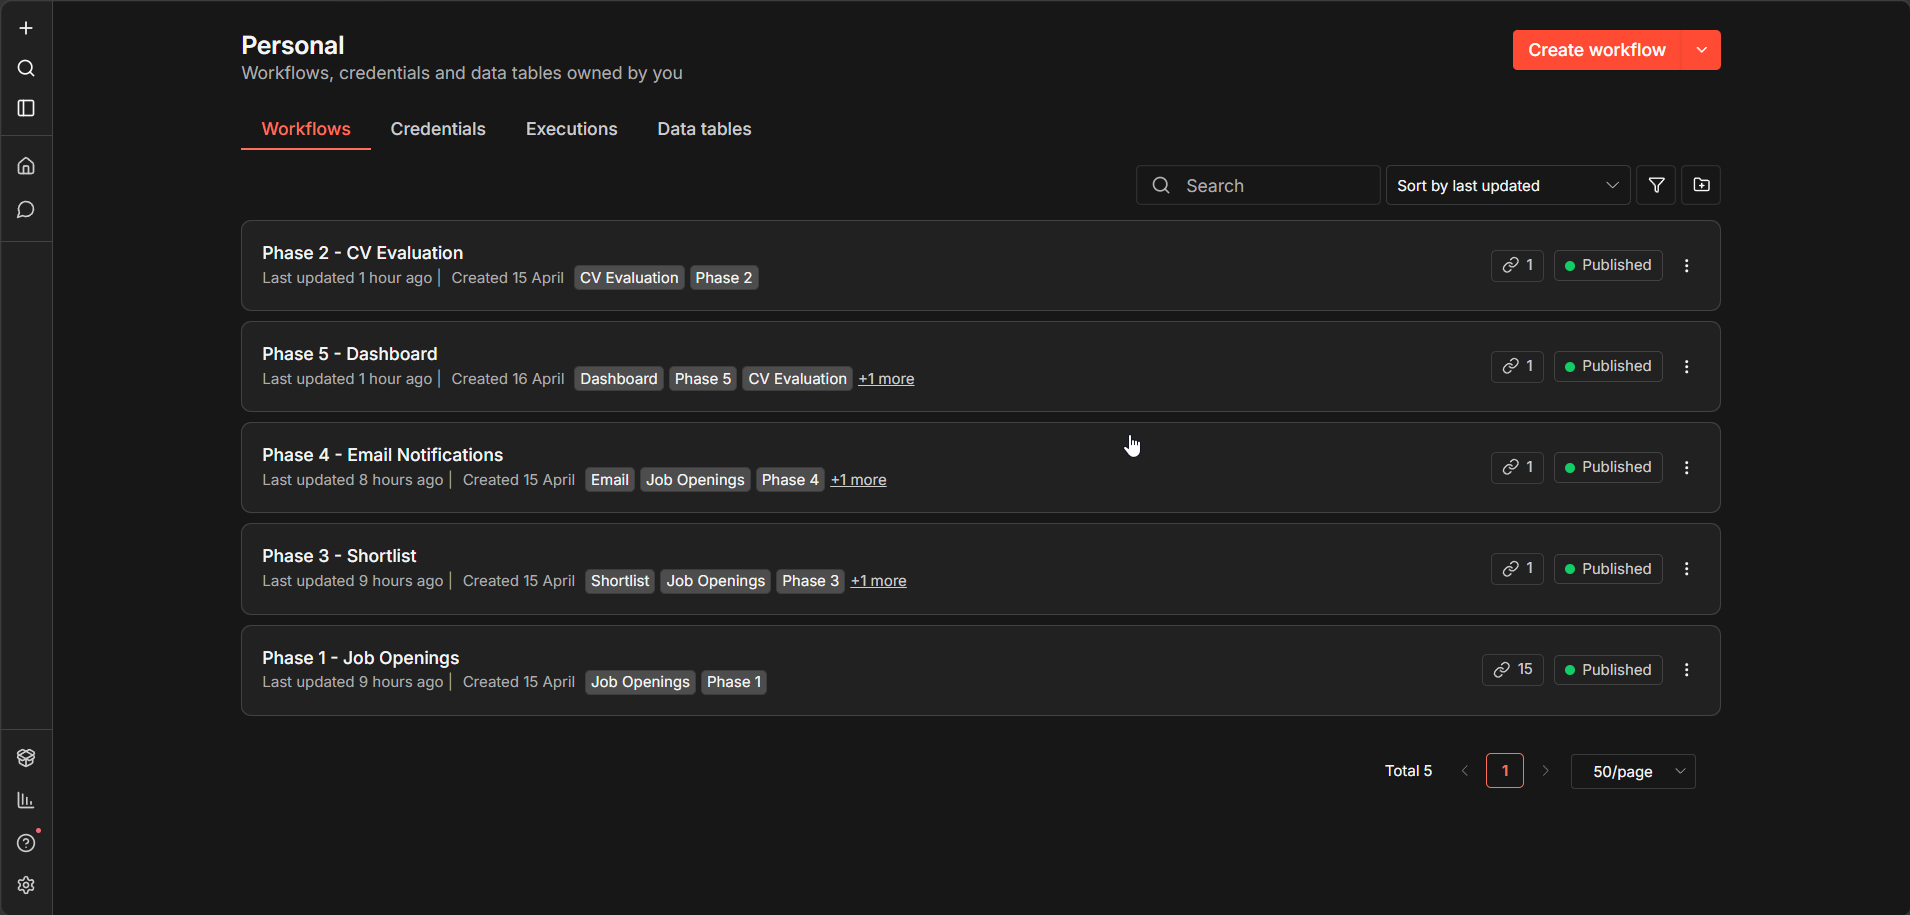
\includegraphics[width=0.9\textwidth]{n8n-workflows.png}
    \caption{The n8n workspace with the five workflows that power the application. Each workflow is tagged by phase and is currently published and active.}
\end{figure}

\begin{figure}[H]
    \centering
    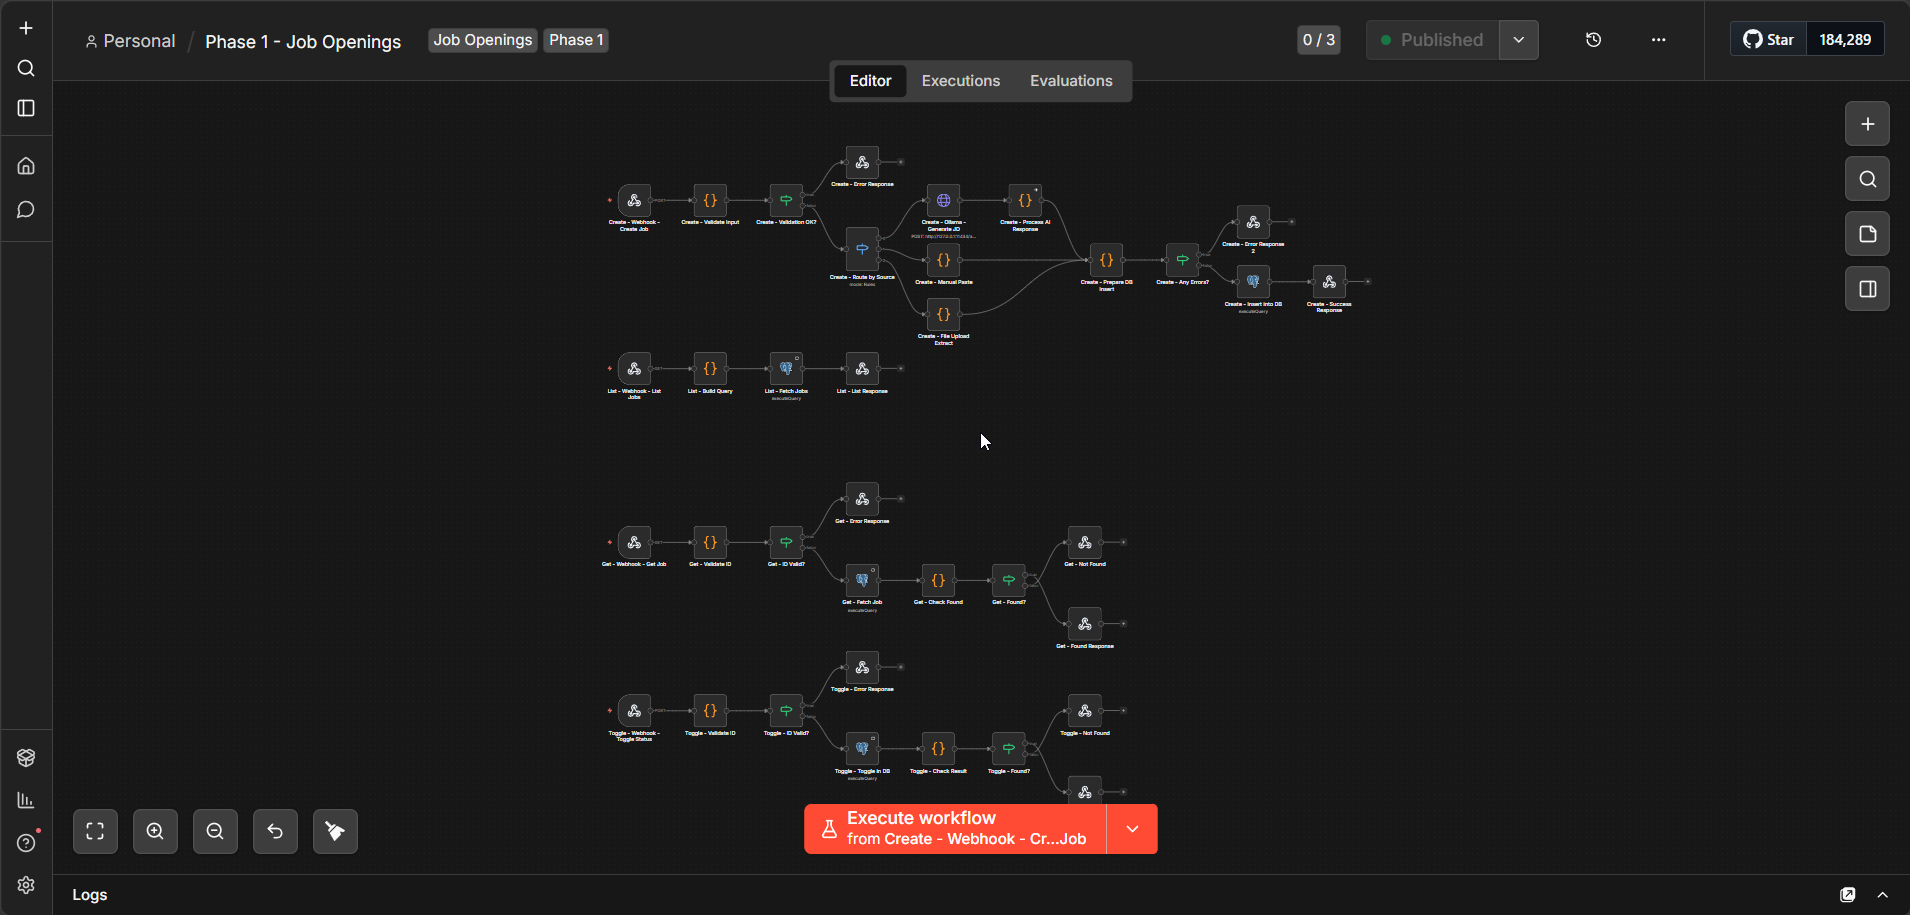
\includegraphics[width=0.9\textwidth]{n8n-editor.png}
    \caption{Inside one workflow (Phase 1, Job Openings). Each block is a step such as validation, database access, or response shaping. Editing the logic is visual, which makes future changes faster and easier to review.}
\end{figure}

% =====================================================
% FRONTEND FUNCTIONALITIES
% =====================================================
\section{Frontend Functionalities}

The HR user sees one single-page application with five tabs. Selecting a job in any tab carries that selection over to the other tabs through a persistent header badge, so context is never lost.

\subsection{Dashboard}

The Dashboard gives a snapshot of hiring activity for the selected job. It shows counts of candidates at each stage of the funnel, the average and top evaluation scores, and a status breakdown.

\begin{figure}[H]
    \centering
    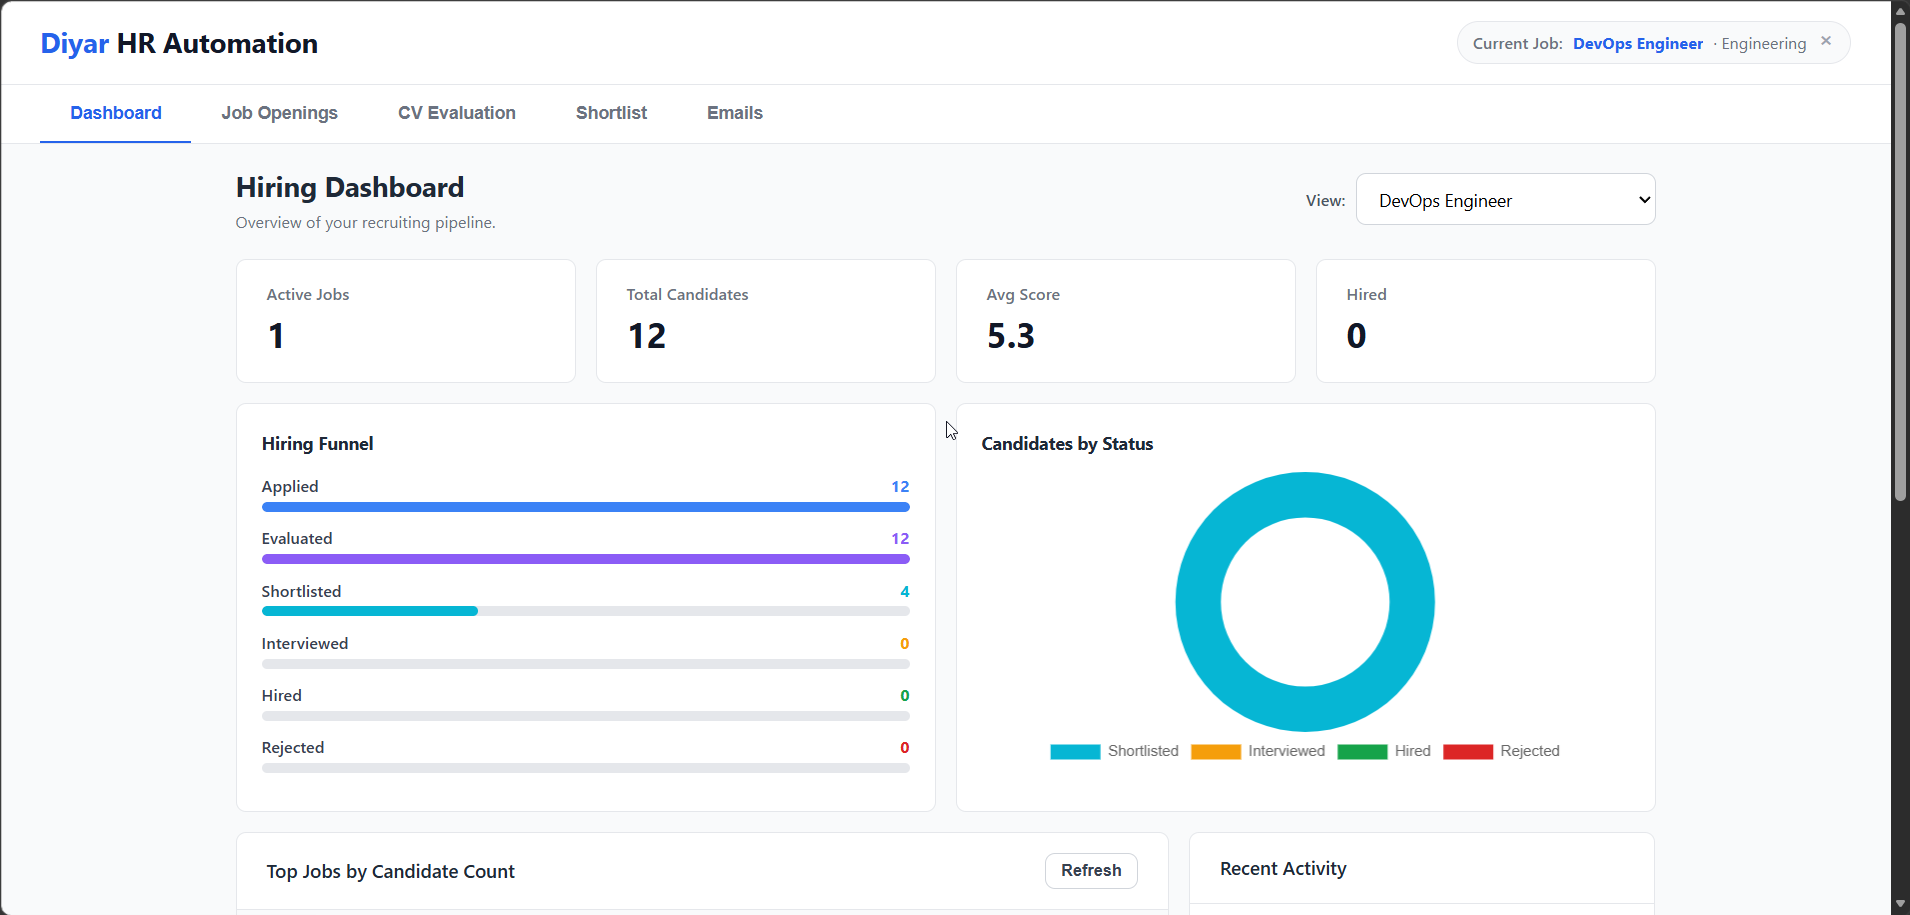
\includegraphics[width=\textwidth]{dashboard.png}
    \caption{Dashboard view for the DevOps Engineer role. At a glance the user can see 12 candidates applied, 12 were evaluated, 4 were shortlisted, and 8 were rejected.}
\end{figure}

\subsection{Job Openings}

Job openings are created through a short two-step wizard. The user enters the basic information first, then provides a job description either by writing it manually, uploading a file, or asking the local AI model to draft one.

\begin{figure}[H]
    \centering
    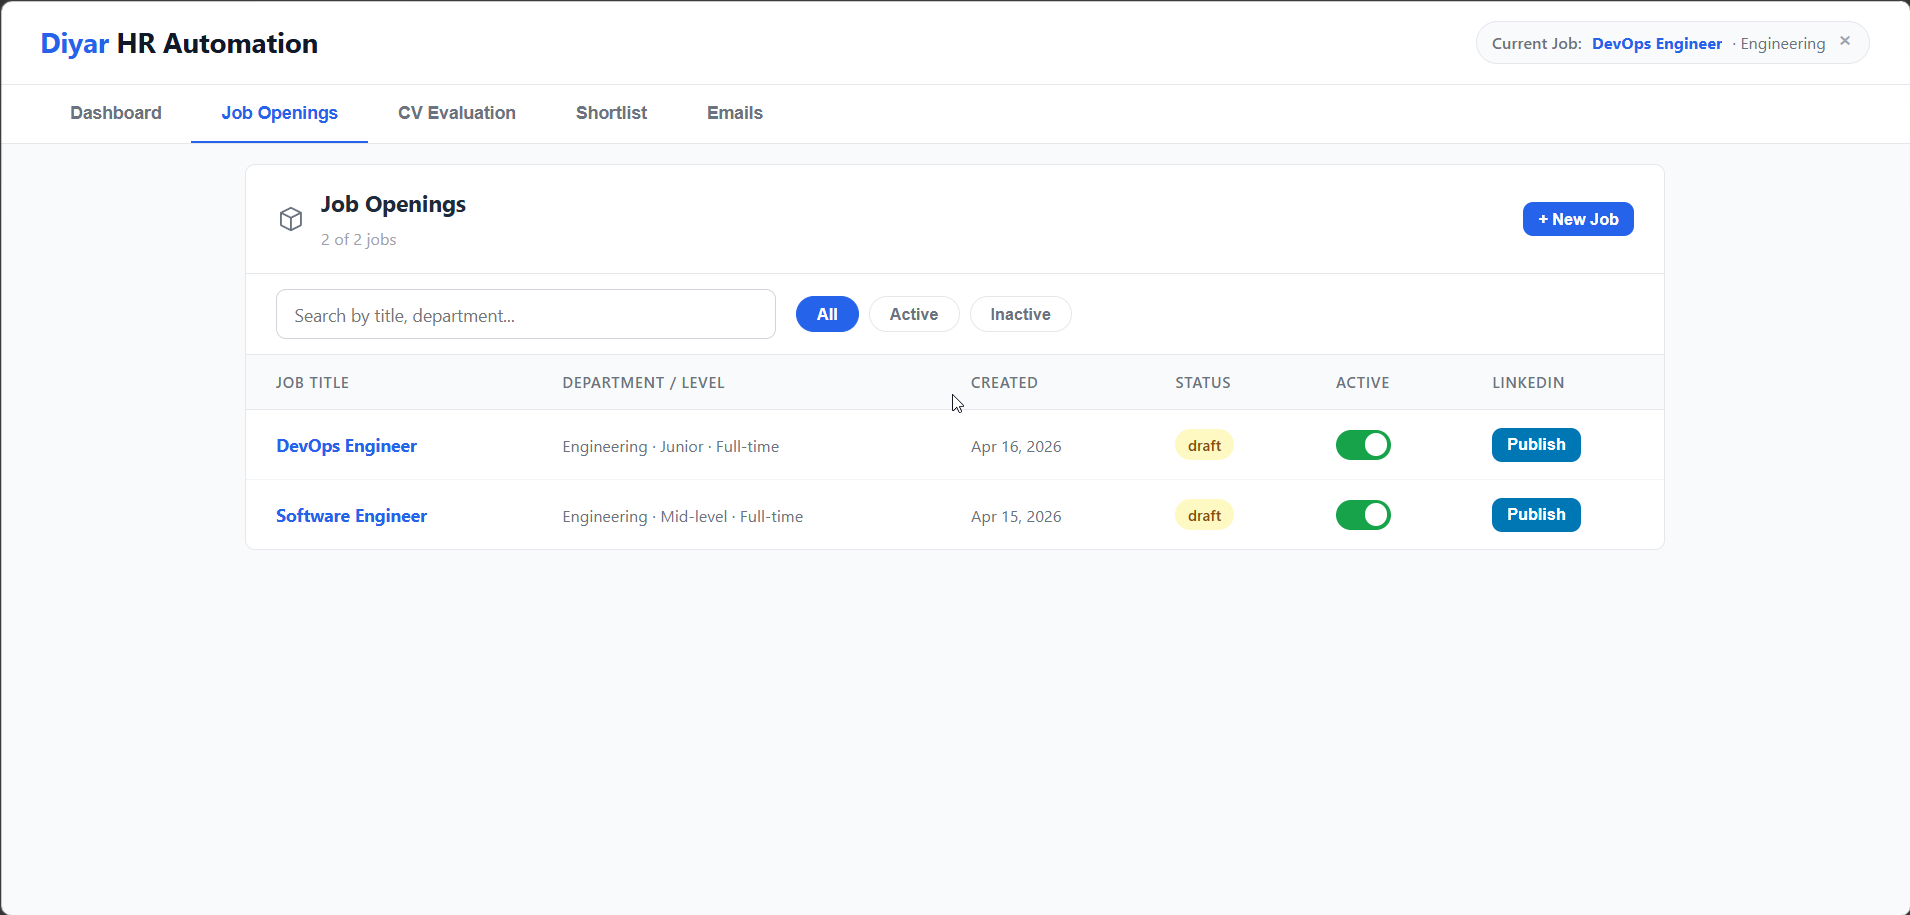
\includegraphics[width=\textwidth]{jobs.png}
    \caption{The Job Openings list. Each row can be activated or deactivated with a toggle, and the Publish LinkedIn button marks the job ready for publishing (outbound publishing itself is planned for a later phase).}
\end{figure}

\subsection{CV Evaluation Wizard}

The evaluation flow is a four-step wizard: choose the job, set the scoring criteria, upload CVs, and review results. The steps are revisitable at any time, so the user can adjust criteria and re-evaluate without starting over.

\subsubsection*{Step 2a, Criteria written by hand}

The user can paste or type the criteria directly. The right-hand column holds one editable draft that every source of criteria feeds into.

\begin{figure}[H]
    \centering
    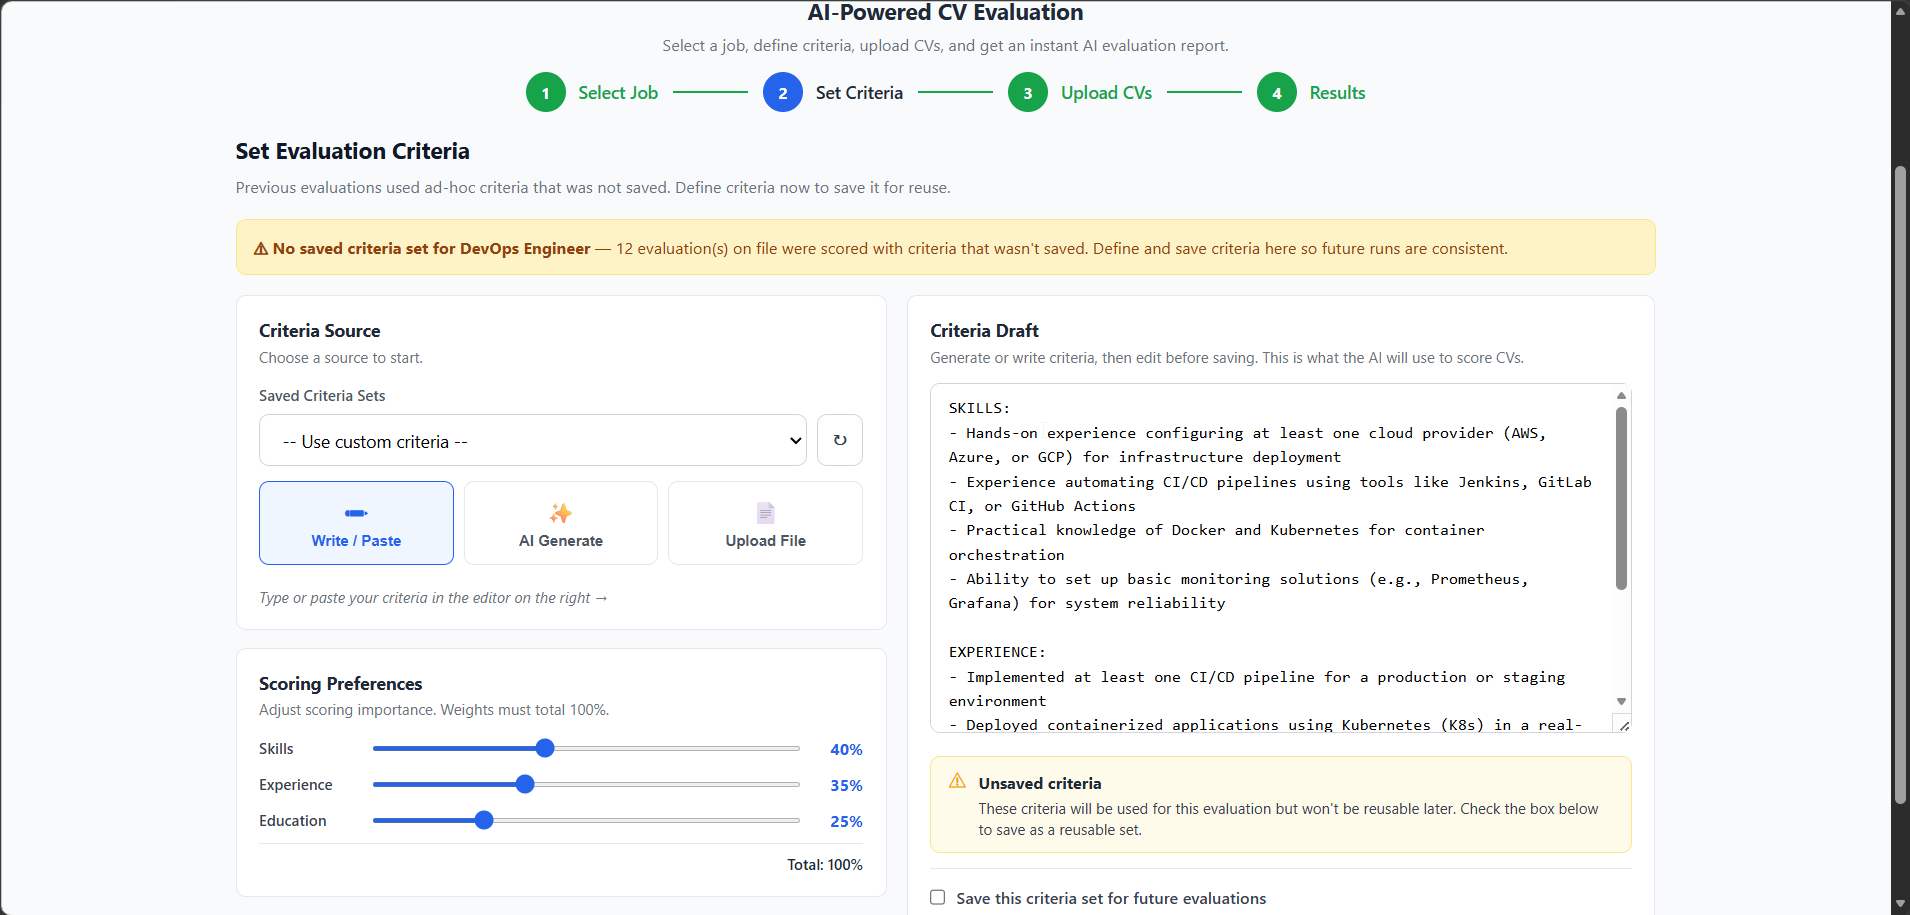
\includegraphics[width=\textwidth]{criteria-write.png}
    \caption{Writing criteria manually. The scoring weights for skills, experience, and education are set on the left and must add up to 100 percent. The amber banner warns the user when a criteria set has not yet been saved.}
\end{figure}

\subsubsection*{Step 2b, Criteria generated by AI}

When the user selects the AI option, they can add extra context such as emphasis on security or collaboration. Clicking Generate asks the local model to propose a criteria list, which then lands in the same draft area ready for edits.

\begin{figure}[H]
    \centering
    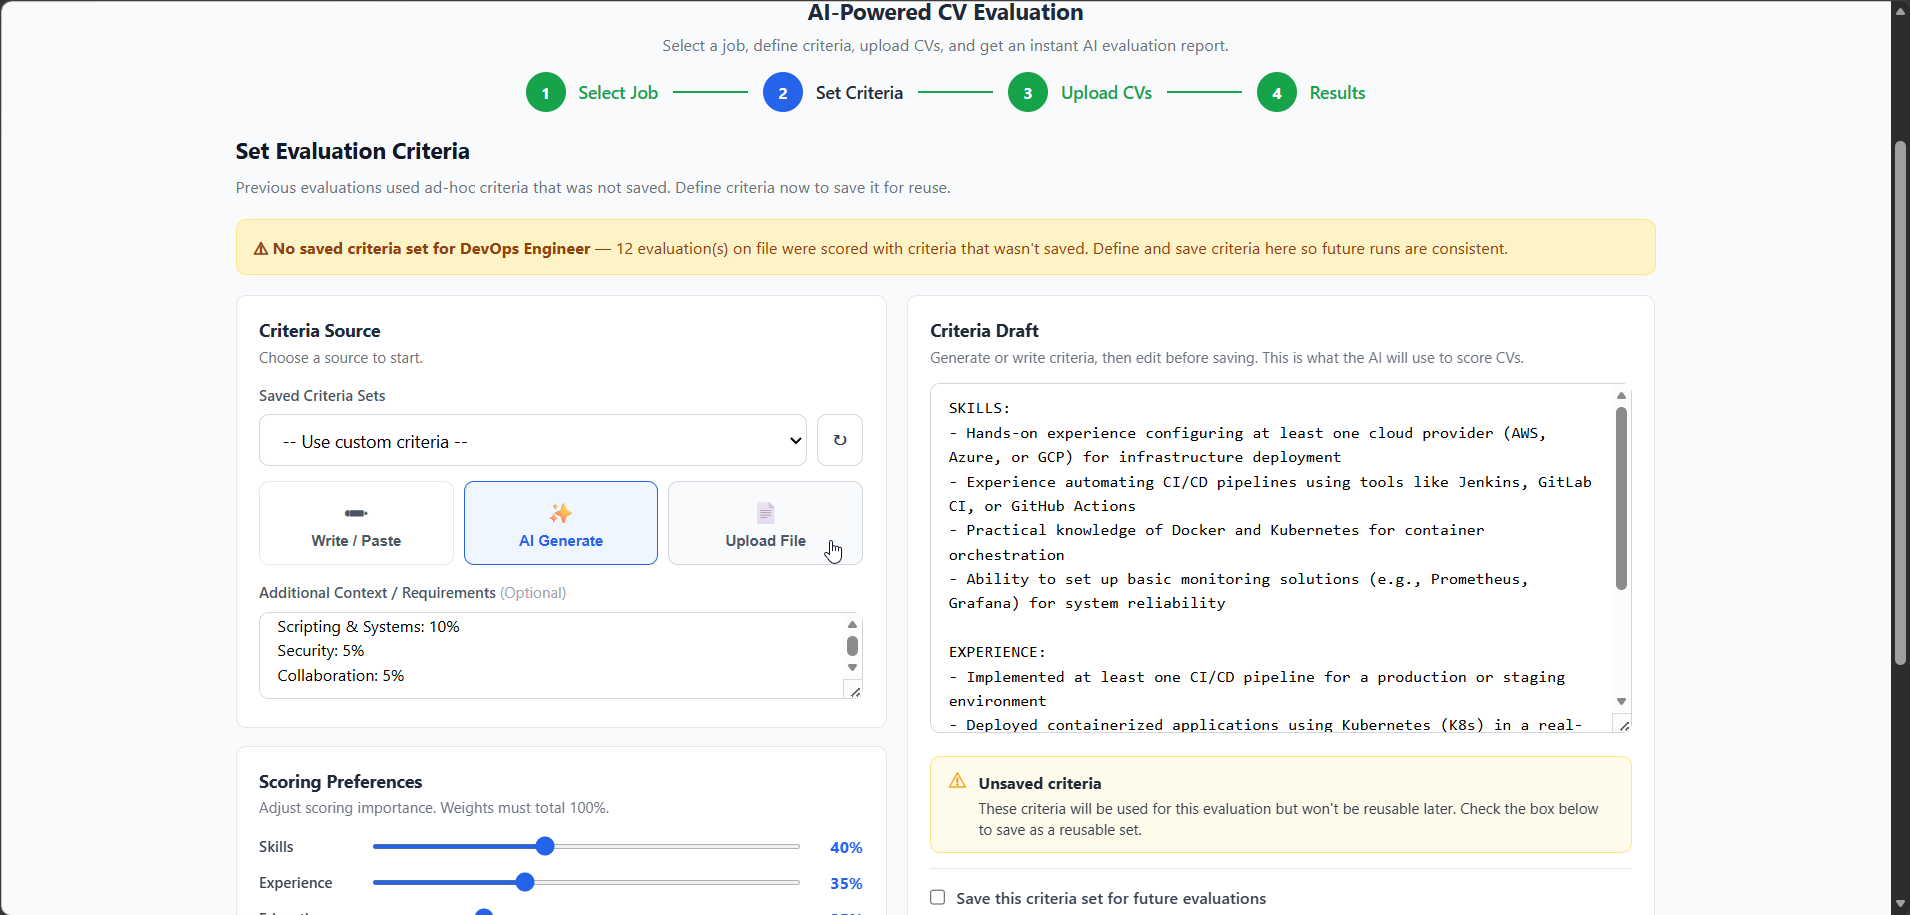
\includegraphics[width=\textwidth]{criteria-ai.png}
    \caption{AI-assisted criteria generation. The additional context box lets HR nudge the model toward specific priorities without writing the full criteria from scratch.}
\end{figure}

\subsubsection*{Step 3, Uploading CVs}

Candidates are added by dragging PDF or text files into the drop zone. Text is extracted in the browser so no CV leaves the laptop. Duplicate candidates are detected on upload.

\begin{figure}[H]
    \centering
    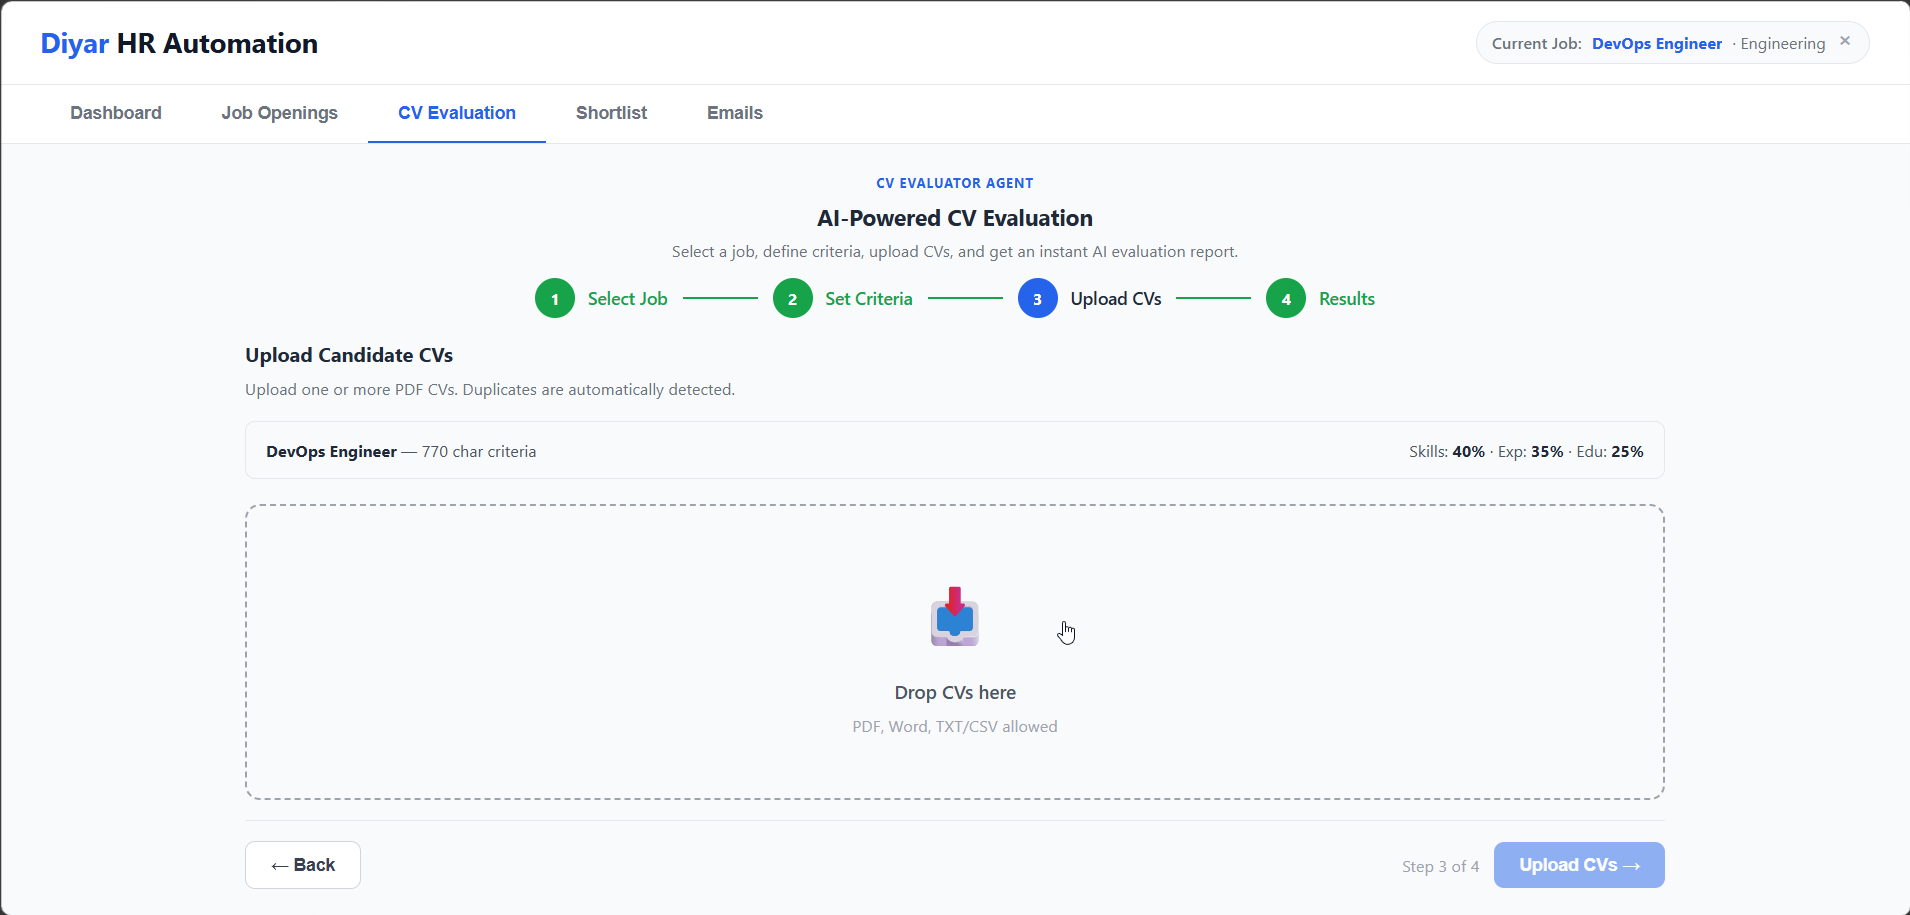
\includegraphics[width=\textwidth]{upload.png}
    \caption{The upload step for a chosen job. The header reminds the user of the job, the criteria preview, and the weights that will be used for evaluation.}
\end{figure}

\subsubsection*{Step 4, Results}

Each candidate receives an overall score and per-dimension scores. The table stays short and scannable; the full reasoning, strengths, and weaknesses appear in a detail view when the user clicks through.

\begin{figure}[H]
    \centering
    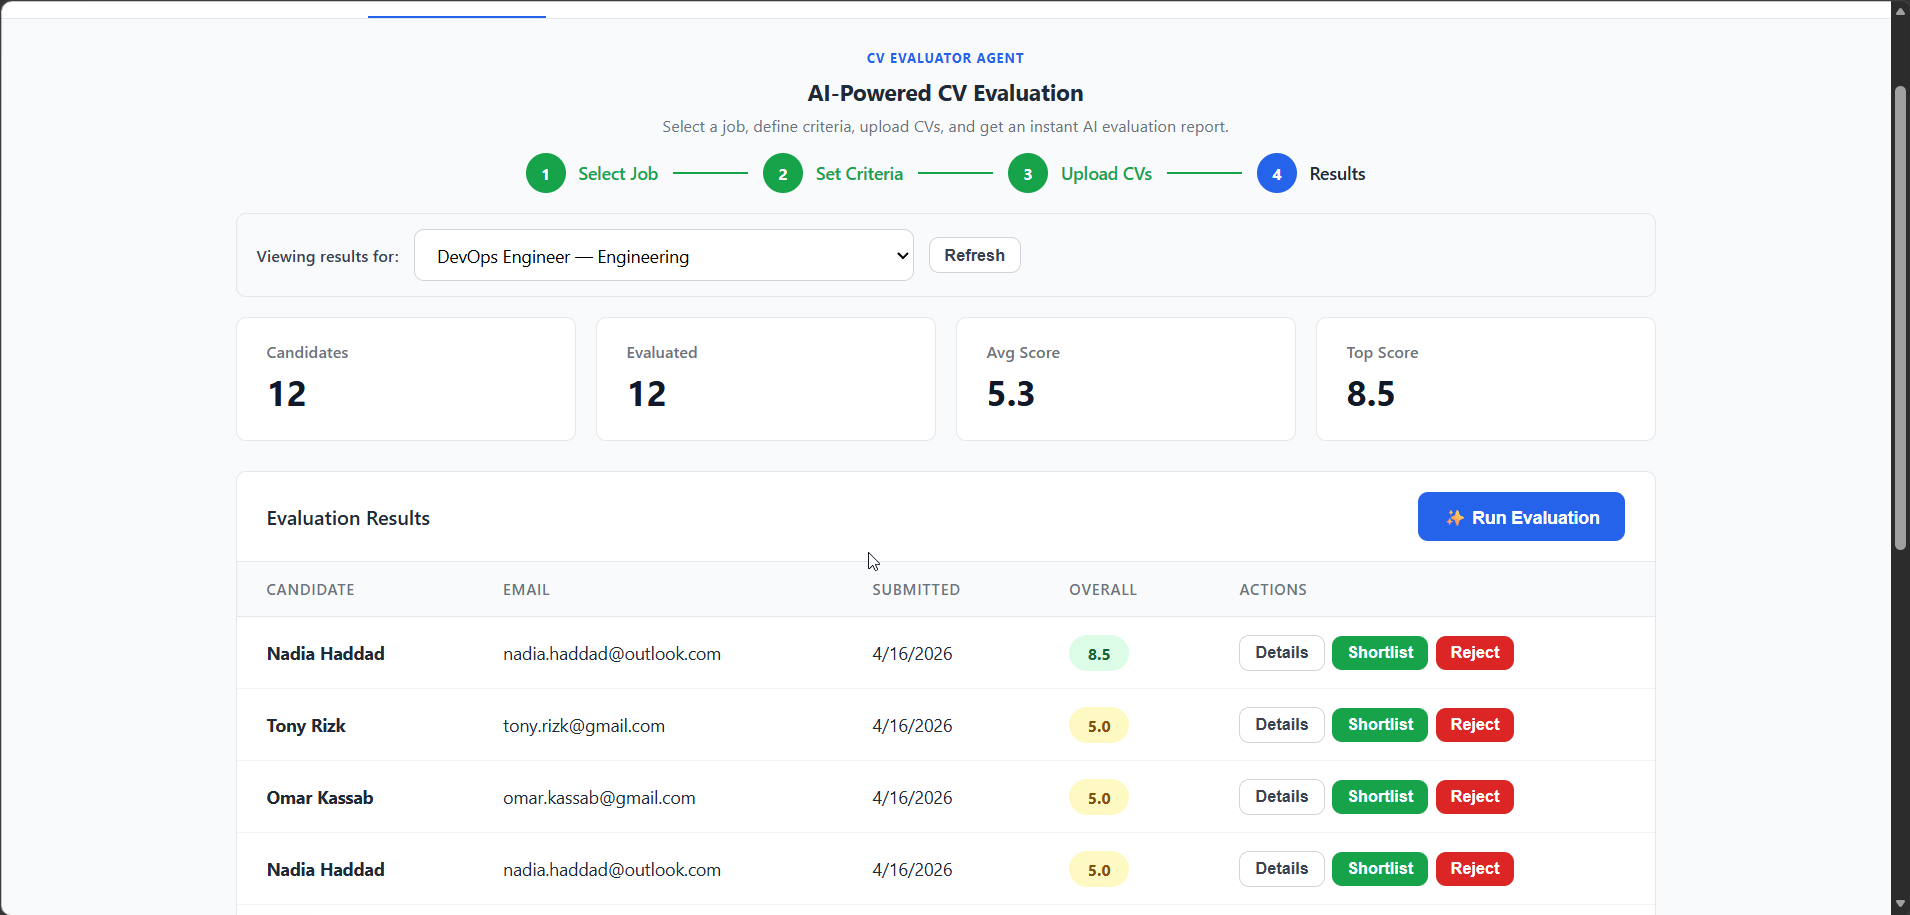
\includegraphics[width=\textwidth]{results.png}
    \caption{Evaluation results sorted by overall score. From here the user can shortlist a promising candidate, reject one, or open the detail view to read the AI reasoning.}
\end{figure}

\subsection{Shortlist and Interview Tracking}

Shortlisted candidates move into a tracking page where HR can mark them as interviewed, hired, or rejected. Status updates happen in place, without reloading the whole page.

\begin{figure}[H]
    \centering
    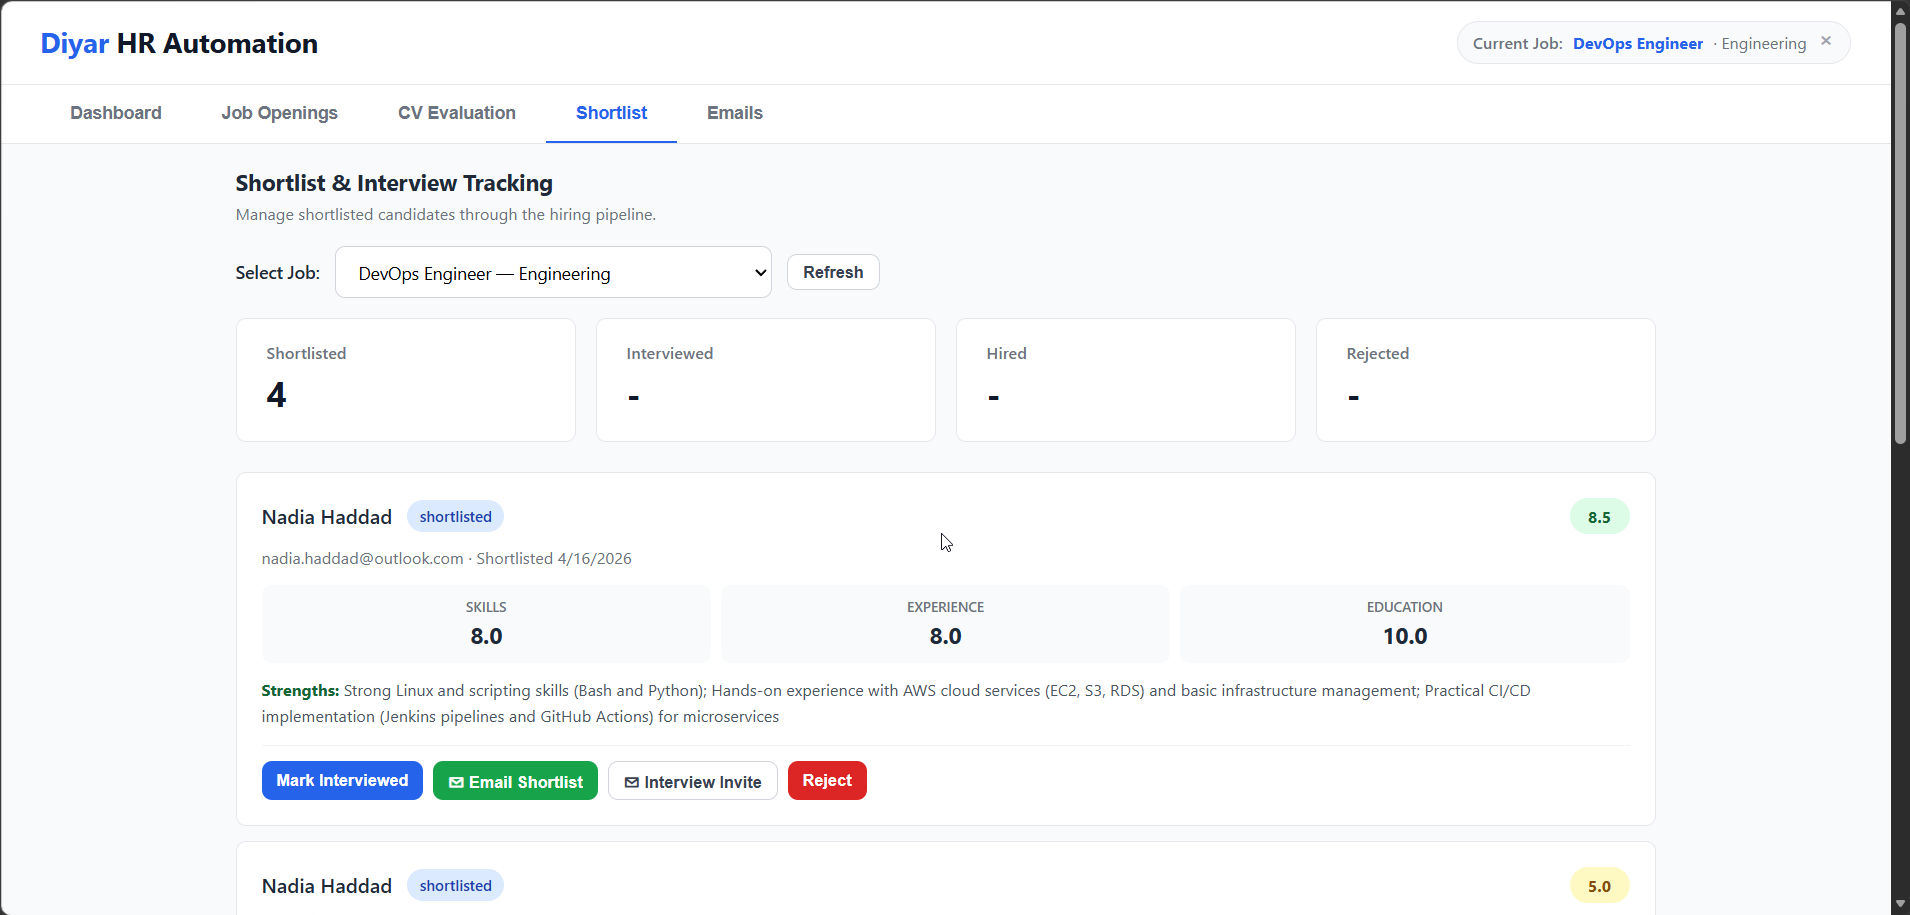
\includegraphics[width=\textwidth]{shortlist.png}
    \caption{A shortlisted candidate card. The per-dimension scores, strengths summary, and next-step buttons (Mark Interviewed, Email Shortlist, Interview Invite, Reject) are all within one click.}
\end{figure}

\subsection{Emails}

Every email the system sends is logged with recipient, subject, timestamp, type, and delivery status. The top of the page shows whether the SMTP connection is healthy, so the HR user can tell at a glance whether outgoing mail is working.

\begin{figure}[H]
    \centering
    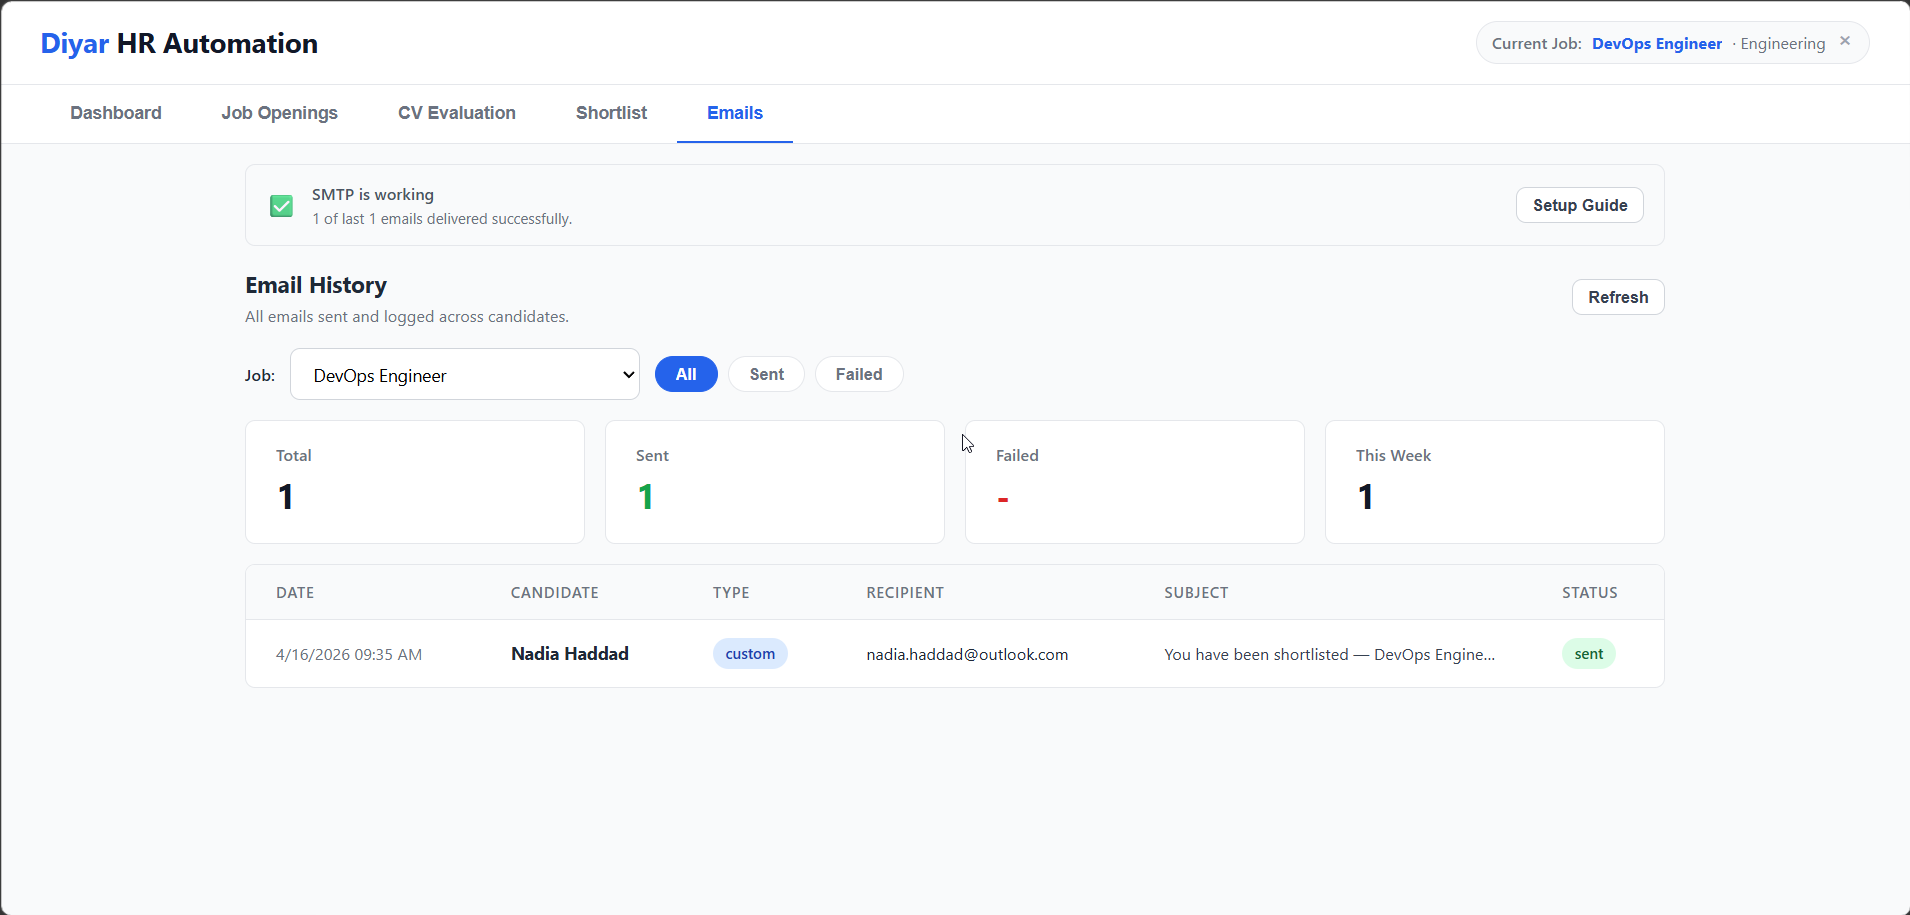
\includegraphics[width=\textwidth]{emails.png}
    \caption{Email history with live SMTP health. Totals, sends, failures, and weekly counts appear as small cards above the log.}
\end{figure}

% =====================================================
% WHAT IS DONE
% =====================================================
\section{What Has Been Delivered}

The following pieces are functional and in daily use across the demo:

\begin{itemize}
    \item Job opening lifecycle with AI-assisted description drafting and activation toggles.
    \item CV intake, in-browser PDF parsing, duplicate detection, and AI evaluation with configurable weights.
    \item Saved criteria sets per job so previous evaluation setups can be reused.
    \item Shortlist tracking with four statuses (shortlisted, interviewed, hired, rejected).
    \item Editable email composer for every candidate-facing message, with logging and SMTP health monitoring.
    \item Cross-tab selected-job context and a one-command startup script for the full stack.
\end{itemize}

% =====================================================
% PLANS BEFORE FINALIZATION
% =====================================================
\section{Planned Work Before Finalization}

The remaining tasks fall into four groups, listed in the order I plan to tackle them.

\subsection{Reliability and Polish}

\begin{itemize}
    \item Tighten the CV parser so multi-column and scanned PDFs extract cleanly.
    \item Add a test-connection and send-test button to the Emails page so SMTP can be verified in-app.
\end{itemize}

\subsection{Feature Completion}

\begin{itemize}
    \item Finish the LinkedIn publish flow (button already on the page, currently a placeholder).
    \item Add an email template manager with reusable subject and body templates.
    \item Extend the dashboard with a time-to-hire metric and a source-of-hire chart.
\end{itemize}

\subsection{Quality and Scoring Improvements}

\begin{itemize}
    \item Split the CV scoring prompt into per-dimension calls for more consistent scores.
    \item Add a side-by-side comparison view for two or more candidates.
\end{itemize}

\subsection{Handover Readiness}

\begin{itemize}
    \item Short video walkthrough of every tab for new HR users.
    \item Packaged launcher that installs missing dependencies on a fresh machine in one click.
\end{itemize}

% =====================================================
% CLOSING
% =====================================================
\section{Closing Note}

To be clear, this is still a proof of concept and there is meaningful work ahead before it is production-ready. What has been built proves the approach works end to end and gives us a solid base to iterate on, but the items in the previous section are real and will need attention before a full rollout.

This is the progress report for the work done so far, and I am ready to demo the project live on Sunday. Please let me know what time works for you and Mr. Ziad so I can walk you through everything that has been built.

\end{document}
